% MDPI Remote Sensing submission package
% Template basis: MDPI v6 class dated 13 March 2026.
\documentclass[remotesensing,article,submit,pdftex,moreauthors]{Definitions/mdpi}

\usepackage{array}
\usetikzlibrary{positioning,arrows.meta}

\newcommand{\method}{BG-RFM}

\firstpage{1}
\makeatletter
\setcounter{page}{\@firstpage}
\makeatother
\pubvolume{1}
\issuenum{1}
\articlenumber{0}
\pubyear{2026}
\copyrightyear{2026}
\datereceived{}
\daterevised{}
\dateaccepted{}
\datepublished{}

\Title{Background-Guided Residual Flow Matching for Multi-Constraint Seismic Velocity Model Building}

\ifdefined\BLINDREVIEW
\Author{Anonymous Author(s)}
\AuthorNames{Anonymous Author(s)}
\address{Affiliations withheld for blind review.}
\corres{Correspondence information withheld for blind review.}
\else
\Author{[AUTHOR NAMES AND AFFILIATION MARKERS]}
\AuthorNames{[AUTHOR NAMES]}
\address{[AFFILIATIONS --- include department/institution/city/postal code/country and author e-mails as required.]}
\corres{Correspondence: [CORRESPONDING AUTHOR NAME AND EMAIL]}
\fi

\abstract{Initial velocity model building benefits from heterogeneous geophysical constraints that describe different aspects of the subsurface. RMS velocity and sparse wells provide strong information about large-scale velocity magnitude, whereas post-stack migrated images and interpreted horizons provide dense structural cues. Most learned approaches nevertheless fuse these observations and assign the complete velocity field to a single predictor or generator. We propose Background-Guided Residual Flow Matching (BG-RFM), which explicitly separates reconstruction responsibilities while retaining multimodal conditioning. A role-aware condition encoder provides background-oriented and structure-oriented interfaces. The background branch deterministically predicts a smooth velocity component, and the residual branch applies conditional Flow Matching to the correction relative to that prediction. Crucially, the same predicted background defines the residual target during training, conditions the residual vector field, and is reused in final velocity composition, yielding a prediction-consistent reconstruction path. We evaluate the method on eight OpenFWI subsets using RMS velocity, post-stack migrated images, horizons, and sparse wells under a common 33,600-record held-out protocol. On this unified benchmark, the proposed model achieves an RMSE of 0.0269 and an SSIM of 0.9916 with 10.6M trainable parameters. The results support a parameter-compact formulation that allocates deterministic estimation to background recovery and generative transport to the remaining correction.}
\keyword{initial velocity model building; seismic velocity reconstruction; Flow Matching; multimodal geophysical constraints; residual generative modeling; OpenFWI}
\addhighlights{yes}
\renewcommand{\addhighlights}{%
\noindent\textbf{What are the main findings?}
\begin{itemize}[labelsep=2.5mm,topsep=-3pt]
\item Role-aware conditioning separates background and residual reconstruction responsibilities.
\item The predicted background is reused for residual definition, residual conditioning, and final composition.
\end{itemize}\vspace{3pt}
\textbf{What is the implication of the main finding?}
\begin{itemize}[labelsep=2.5mm,topsep=-3pt]
\item BG-RFM provides a parameter-compact, prediction-consistent generative formulation for multi-constraint seismic velocity model building.
\end{itemize}
}

\begin{document}

\section{Introduction}

A reliable initial velocity model is a prerequisite for seismic imaging and waveform-based inversion because velocity controls travel-time kinematics and the positioning and focusing of subsurface structures \citep{stolt1978migration,tarantola1984inversion,virieux2009overview}. Full-waveform inversion can recover detailed velocity structure, but its optimization remains sensitive to the starting model, acquisition coverage, missing low-frequency information, and cycle skipping \citep{bunks1995multiscale,virieux2009overview}. Initial velocity model building therefore remains an important problem even when sophisticated downstream inversion tools are available.

Data-driven velocity reconstruction provides a complementary route by amortizing the mapping from observations to a velocity model \citep{yang2019deeplearning,wu2020inversionnet,deng2022openfwi}. Most benchmark methods are developed around one dominant observation type, especially multi-shot seismic data. In practical interpretation workflows, however, several processed or interpreted products may already be available. RMS velocity carries smooth kinematic and absolute-scale information; post-stack migrated images provide spatially dense reflector geometry; interpreted horizons localize interfaces; and wells offer sparse but high-confidence velocity anchors. These observations are heterogeneous in physical meaning, sampling domain, density, and uncertainty.

A common strategy is to encode the available observations, fuse their features, and predict or generate the complete velocity field with one downstream estimator. The estimator may be a deterministic convolutional network, an adversarial generator, a latent model, or a diffusion/flow-based model. This design can exploit multimodal information, but it leaves the reconstruction responsibility implicit: the same estimator must recover both a comparatively smooth velocity background and the remaining structural correction. Increasing the capacity of a fused full-field model does not by itself specify which information should control which part of the reconstruction.

We formulate the problem differently. The key observation is not that the modalities are universally separable, but that they provide complementary tendencies that can support different reconstruction roles. We therefore learn two condition interfaces from all available modalities: one used to predict a deterministic background velocity and another used to guide residual reconstruction. The predicted background is then treated as a first-class variable rather than an intermediate feature. It defines the residual target, provides context to the residual generator, and is added back to the generated correction.

This leads to Background-Guided Residual Flow Matching (\method). Given multimodal observations, the method first predicts a background field $\hat B$. Instead of transporting the complete velocity model, it learns a conditional Flow Matching vector field for the prediction-relative residual $R_{\hat B}=V-\hat B$. The same $\hat B$ is reused in the residual supervision, residual conditioning, and final composition $\hat V=\hat B+\hat R$. This prediction-consistent construction aligns the residual task used during training with the background available at inference and gives the deterministic and generative branches explicit responsibilities.

The contributions of this study are threefold:
\begin{itemize}
    \item We develop a role-aware multi-source conditioning framework for RMS velocity, post-stack migrated images, interpreted horizons, and sparse wells. Every available modality can contribute to both learned roles, while the downstream interfaces explicitly distinguish background prediction from structural/residual guidance.
    \item We introduce prediction-consistent residual Flow Matching for seismic velocity model building. The same predicted background is used to define the residual target, condition the residual vector field, and compose the final velocity estimate, directly coupling residual learning to the background that will be available at inference.
    \item We develop a parameter-compact prediction-consistent generative formulation for structured velocity reconstruction and evaluate it under a unified held-out OpenFWI protocol against adapted deterministic and generative references. The contribution is the reconstruction organization and compact parameterization rather than overall benchmark dominance.
\end{itemize}

The resulting perspective is simple: \emph{predict the background; transport the prediction-relative correction}. This responsibility allocation, rather than a claim of universal frequency--uncertainty separation, is the central design principle evaluated in the remainder of the paper.

\section{Related Work}

\subsection{Learning-Based Seismic Velocity Model Building}

Learning-based seismic inversion has developed from direct convolutional mappings between seismic measurements and subsurface velocity toward larger encoder--decoder, attention-based, and structured inverse architectures. Fully convolutional approaches demonstrated the feasibility of amortized velocity inversion \citep{yang2019deeplearning}, while InversionNet established a widely used OpenFWI benchmark \citep{wu2020inversionnet,deng2022openfwi}. Later methods explored alternative architectures and physical priors, and UPFWI introduced an unsupervised/physics-coupled formulation based on wave-equation consistency \citep{jin2022upfwi}. These studies differ substantially in input measurements and optimization objectives. Accordingly, the present work distinguishes source-native literature context from the controlled matched-input adaptations used in the journal comparison.

\subsection{Generative Modeling for Velocity Reconstruction}

Generative models provide an alternative to deterministic regression when the inverse mapping contains structurally complex or multimodal variation. Adversarial generators can encourage sharp outputs but introduce adversarial optimization. Diffusion and score-based models learn iterative denoising or score fields \citep{ho2020ddpm,song2021scorebased}, and latent diffusion reduces generative cost by operating in a compressed representation \citep{rombach2022ldm}. Flow Matching and rectified flow instead learn continuous vector fields that transport a simple base distribution to a target distribution \citep{lipman2023flowmatching,liu2023rectifiedflow}. Recent geophysical work has applied diffusion-style modeling to controllable velocity synthesis and inversion \citep{wang2024controllable}. Most such formulations still treat the complete target field as the generative variable. \method{} instead assigns deterministic estimation to the background and applies generative transport only to the correction relative to the predicted background.

\subsection{Heterogeneous Geophysical Constraint Integration}

Velocity model building can use information beyond raw shot gathers. RMS velocity constrains smooth kinematics and velocity scale \citep{dix1955velocities}; migrated images provide reflector geometry \citep{stolt1978migration}; horizons summarize interpreted interfaces; and wells provide sparse local velocity control. Multimodal learning offers general tools for alignment, fusion, and missing-modality handling \citep{baltrusaitis2019multimodal,tian2020cmc,saporta2024symile}. The remaining question is not only how to fuse heterogeneous observations, but how to assign reconstruction responsibilities after fusion.

This is the gap addressed here. Existing learned inversion methods generally predict the full velocity field directly or condition a full-field generative model globally. \method{} uses all available modalities to learn role-aware condition interfaces, but explicitly assigns deterministic background recovery and generative residual transport different downstream responsibilities. The two branches are coupled through a shared predicted-background reference, rather than through a hard one-modality/one-role partition.

\section{Materials and Methods}

\subsection{Problem Formulation and Observation Contract}

Let
\[
X=\{M,H,V_{\mathrm{rms}},W\}
\]
denote the available multimodal observations, where $M$ is the post-stack migrated image, $H$ is an interpreted-horizon map, $V_{\mathrm{rms}}$ is the RMS-velocity field, and $W$ is a sparse well-velocity map. The target is the depth-domain velocity model
\[
V\in\mathbb{R}^{1\times70\times70}.
\]
RMS velocity and the migrated image are represented on a $1000\times70$ time--lateral grid, whereas horizons, wells, and the target use the $70\times70$ depth grid. Only observed quantities and their masks cross the public inference boundary; target-derived decomposition quantities are restricted to training supervision or post-hoc diagnostics.


\begin{table}[H]
\caption{Multimodal task definition used in the Remote Sensing evaluation.\label{tab:task-contract}}
\begin{tabularx}{\textwidth}{lCCC}
\toprule
\textbf{Quantity} & \textbf{Domain} & \textbf{Shape} & \textbf{Role} \\
\midrule
Target velocity $V$ & depth & $1\times70\times70$ & prediction target \\
RMS velocity $V_{\mathrm{rms}}$ & time & $1\times1000\times70$ & kinematic/scale cue \\
Migrated image $M$ & time & $1\times1000\times70$ & structural cue \\
Horizon map $H$ & depth & $1\times70\times70$ & interface cue \\
Sparse well map $W$ & depth & $1\times70\times70$ & local velocity anchor \\
\bottomrule
\end{tabularx}
\end{table}


The benchmark is constructed from FlatVel-A/B, CurveVel-A/B, FlatFault-A/B, and CurveFault-A/B in OpenFWI \citep{deng2022openfwi}. For each reference velocity model, processed/interpreted observations are generated offline to emulate a post-stack model-building workflow. This defines a controlled multimodal benchmark and should not be interpreted as independent field acquisition of every constraint.

\paragraph{RMS velocity.}
For each lateral position, depth samples are mapped to two-way time through
\begin{equation}
t(z,x)=2\int_0^z \frac{1}{V(z',x)}\,\mathrm{d}z',
\end{equation}
and RMS velocity is computed after interpolation to a uniform time grid:
\begin{equation}
V_{\mathrm{rms}}^2(t,x)=\frac{1}{t}\int_0^t v^2(\tau,x)\,\mathrm{d}\tau.
\end{equation}

\paragraph{Post-stack migrated image.}
OpenFWI shot records are processed by common-midpoint grouping, normal-moveout correction using the associated RMS velocity, stacking, and post-stack time migration. The resulting section provides dense structural information on the time--lateral grid.

\paragraph{Horizons and wells.}
The benchmark horizon map is constructed from strong vertical velocity gradients using a fixed quantile rule. Sparse wells retain selected velocity columns together with a binary observation mask. Well locations vary during training and are deterministic for validation and testing under the fixed well seed.

\subsection{Role-Aware Multi-Source Conditioning}

The modalities differ in domain, density, and semantic content, but the network does not impose a hard modality partition. Each modality is encoded into background-oriented and structure-oriented representations,
\begin{equation}
\mathcal E_m(x_m)=\left(Z_m^{\mathrm{bg}},Z_m^{\mathrm{str}},r_m\right),
\end{equation}
where $r_m$ contains learned role-specific reliability scores. Availability, externally supplied quality, and predicted reliability define normalized fusion weights. The two fused interfaces are
\begin{equation}
C_k=\mathcal G_k\left(\sum_{m\in\Omega} w_m^k Z_m^k\right),
\qquad k\in\{\mathrm{bg},\mathrm{str}\},
\end{equation}
with $\Omega$ the observed modality set. In the reported configuration, the background adapter is identity and the structural adapter is a lightweight spatial mapping.

Training-only multimodal alignment, role calibration, and separation terms encourage the two interfaces to preserve complementary information. They do not constitute inference inputs and are not interpreted as a proof that the modalities are physically separable. Full definitions of the auxiliary condition objective are provided in Supplementary Section~S1.


\begin{figure}[H]
\centering
\resizebox{0.95\linewidth}{!}{%
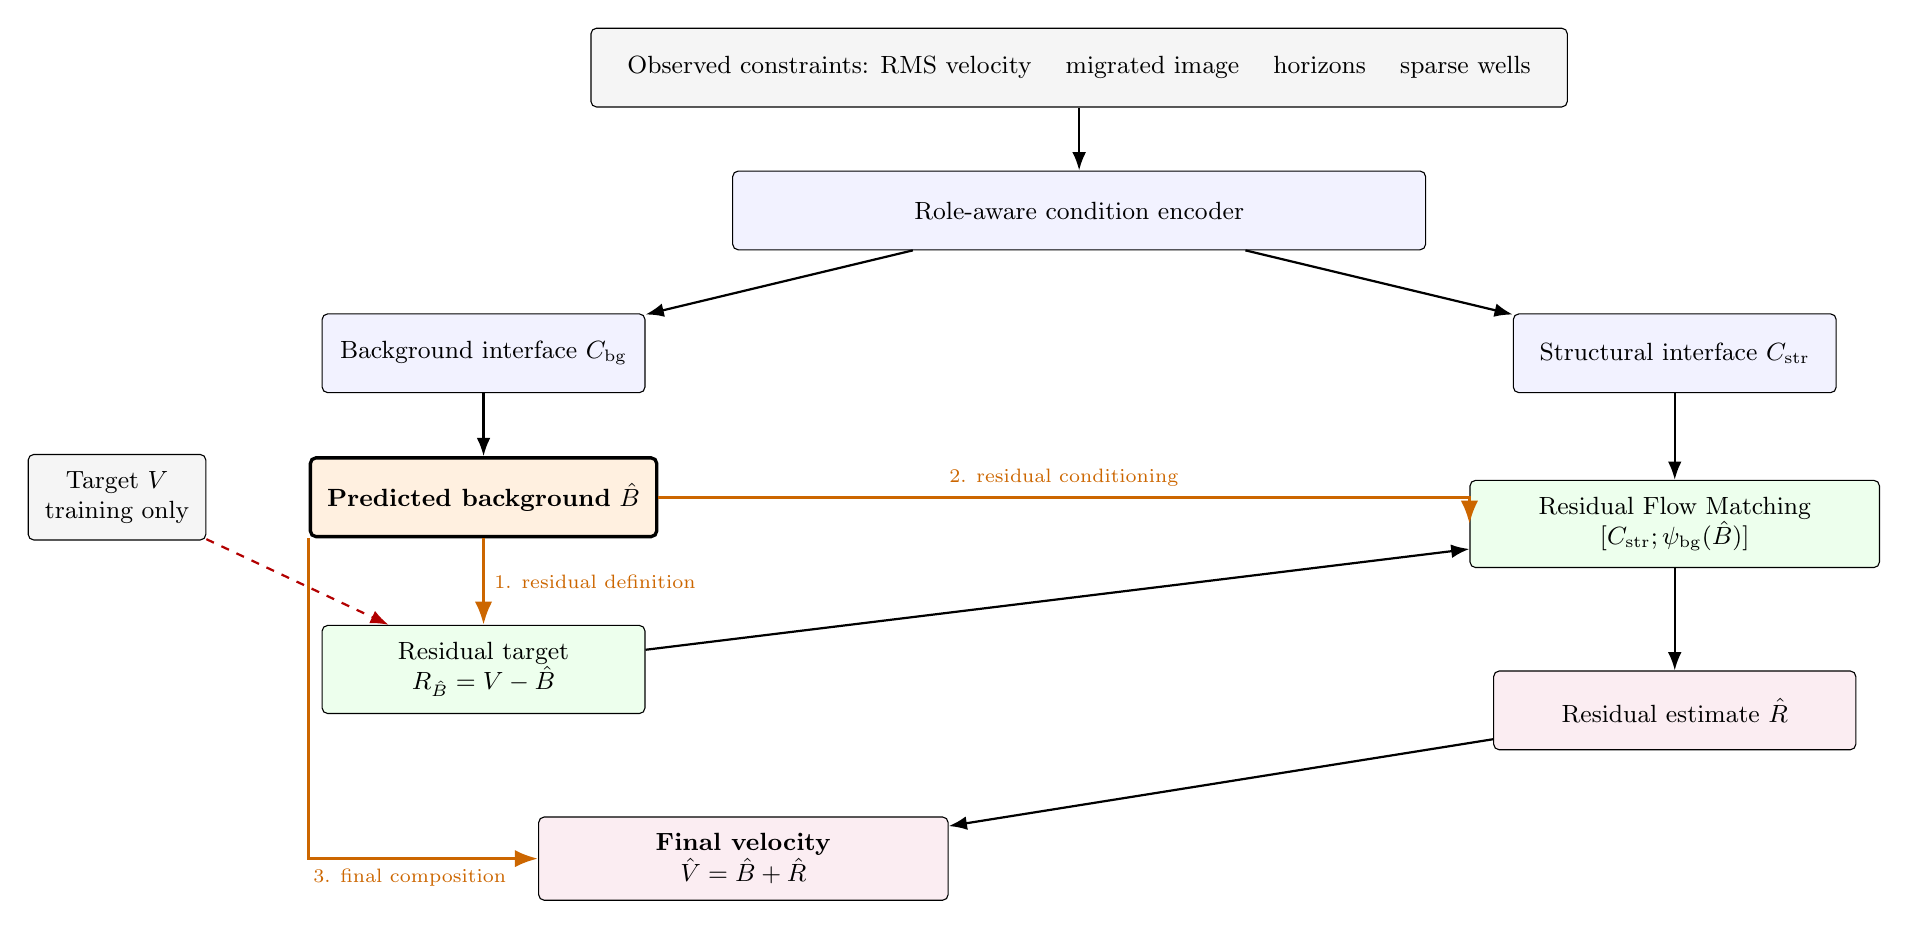
\begin{tikzpicture}[
  font=\small,
  node distance=8mm and 11mm,
  box/.style={draw, rounded corners=2pt, align=center, inner sep=6pt, minimum height=10mm},
  obs/.style={box, fill=gray!8},
  cond/.style={box, fill=blue!5},
  bg/.style={box, fill=orange!12, very thick},
  res/.style={box, fill=green!7},
  outputbox/.style={box, fill=purple!7},
  flow/.style={-Latex, thick},
  reuse/.style={-Latex, very thick, orange!80!black},
  train/.style={-Latex, dashed, thick, red!70!black}
]
\node[obs, minimum width=12.4cm] (obs) {Observed constraints: RMS velocity \quad migrated image \quad horizons \quad sparse wells};
\node[cond, below=of obs, minimum width=8.8cm] (enc) {Role-aware condition encoder};
\node[cond, below left=of enc, minimum width=4.1cm] (cbg) {Background interface $C_{\mathrm{bg}}$};
\node[cond, below right=of enc, minimum width=4.1cm] (cstr) {Structural interface $C_{\mathrm{str}}$};
\node[bg, below=of cbg, minimum width=4.1cm] (bhat) {\textbf{Predicted background} $\hat B$};
\node[obs, left=13mm of bhat, minimum width=2.0cm] (v) {Target $V$\\training only};
\node[res, below=11mm of cstr, minimum width=5.2cm] (fm) {Residual Flow Matching\\$[C_{\mathrm{str}};\psi_{\mathrm{bg}}(\hat B)]$};
\node[res, below=11mm of bhat, minimum width=4.1cm] (rt) {Residual target\\$R_{\hat B}=V-\hat B$};
\node[outputbox, below=13mm of fm, minimum width=4.6cm] (rhat) {Residual estimate $\hat R$};
\node[outputbox, below=13mm of rt, xshift=33mm, minimum width=5.2cm] (final) {\textbf{Final velocity}\\$\hat V=\hat B+\hat R$};

\draw[flow] (obs) -- (enc);
\draw[flow] (enc) -- (cbg);
\draw[flow] (enc) -- (cstr);
\draw[flow] (cbg) -- (bhat);
\draw[flow] (cstr) -- (fm);
\draw[train] (v) -- (rt);
\draw[reuse] (bhat) -- node[right, font=\scriptsize]{1. residual definition} (rt);
\draw[reuse] (bhat.east) -| node[pos=.25, above, font=\scriptsize]{2. residual conditioning} (fm.west);
\draw[flow] (rt) -- (fm);
\draw[flow] (fm) -- (rhat);
\draw[flow] (rhat) -- (final);
\draw[reuse] (bhat.south west) |- node[pos=.72, below, font=\scriptsize]{3. final composition} (final.west);
\end{tikzpicture}}%

\caption{BG-RFM overview. The same predicted background $\hat B$ is reused in three places: it defines the prediction-relative residual target during training, conditions the residual vector field together with $C_{\mathrm{str}}$, and is added back in the final composition. Dashed red arrows denote target-derived training-only information; inference uses observed constraints only.}
\label{fig:bg-rfm-overview}
\end{figure}


\subsection{Deterministic Background Prediction}

A full-resolution U-Net \citep{ronneberger2015unet} predicts
\begin{equation}
\hat B=f_{\mathrm{bg}}(C_{\mathrm{bg}})
\end{equation}
on the velocity grid. A fixed low-pass operator $P_L$ defines the supervision target:
\begin{equation}
\mathcal L_{\mathrm{bg}}
=
\|\hat B-P_L(V)\|_1
+\lambda_{\mathrm{bg},2}\|\hat B-P_L(V)\|_2^2.
\end{equation}
The branch is not intended to produce the final model alone. Its role is to provide a deterministic background estimate and a concrete reference for the remaining correction.

\subsection{Prediction-Consistent Residual Flow Matching}

The residual target is defined relative to the actual predicted background,
\begin{equation}
R_{\hat B}=V-\hat B,
\label{eq:rs_pred_residual}
\end{equation}
rather than an oracle background unavailable at inference. During residual optimization, a stop-gradient copy $\bar B=\mathrm{sg}[\hat B]$ prevents the residual loss from redefining the exclusive optimization responsibility of the background branch.

The residual vector field receives the structural condition and an embedding of the same predicted background,
\begin{equation}
c=[C_{\mathrm{str}};\psi_{\mathrm{bg}}(\bar B)].
\end{equation}
For $t\sim\mathcal U(0,1)$ and $\xi\sim\mathcal N(0,I)$,
\begin{equation}
R_t=(1-t)\xi+tR_{\hat B},
\qquad
u_t=R_{\hat B}-\xi,
\end{equation}
and the Flow Matching objective is
\begin{equation}
\mathcal L_{\mathrm{FM}}
=
\mathbb E\left[
\|v_\theta(R_t,t,c)-u_t\|_2^2
\right].
\end{equation}
Reconstruction-oriented endpoint terms additionally align the sampled residual with the composed velocity estimate; their full form is given in Supplementary Section~S1.

The defining consistency property follows from
\begin{equation}
\hat V=\hat B+\hat R.
\end{equation}
Combining this with Eq.~\eqref{eq:rs_pred_residual} gives
\begin{equation}
\hat V-V=\hat R-R_{\hat B}.
\label{eq:rs_composition_identity}
\end{equation}
Thus final reconstruction error is measured against the residual target defined by the same background used at inference. This identity motivates reusing $\hat B$ for residual supervision, vector-field conditioning, and composition without requiring a universal conditional-entropy argument.

\subsection{Joint Training and Inference}

The joint objective is
\begin{equation}
\mathcal L=
\mathcal L_R+\mathcal L_{\mathrm{bg}}+\lambda_C\mathcal L_C,
\end{equation}
where $\mathcal L_C$ trains the role-aware conditions, $\mathcal L_{\mathrm{bg}}$ trains deterministic background prediction, and $\mathcal L_R$ trains residual transport. The final configuration uses a 192-hidden-channel background U-Net and a 128-hidden-channel FiLM \citep{perez2018film} residual U-Net operating directly on the $70\times70$ velocity grid. The complete model has 10.6M trainable parameters.

At inference, the model receives only the observed modalities and masks, forms $(C_{\mathrm{bg}},C_{\mathrm{str}})$, predicts $\hat B$, integrates the learned residual vector field from the Gaussian base, and returns $\hat V=\hat B+\hat R$. The reported evaluation uses 50 Euler steps. Because this iterative solve requires repeated vector-field evaluations, parameter compactness is not equated with lower wall-clock latency.

\subsection{Experimental Protocol}

The multimodal corpus contains 336,000 aligned records across eight OpenFWI subsets. A deterministic global split of 0.7/0.2/0.1 with split seed 42 yields 33,600 held-out records. Test-time wells are deterministic under well seed 1234. Record identity is fixed by \texttt{dataset\_id}, \texttt{dataset\_name}, and \texttt{source\_sample\_index}.

The authoritative matched-input comparison re-evaluates retained checkpoints on the same held-out membership, normalization, and evaluator. The comparison contains adapted InversionNet, adapted VelocityGAN, a supervised multimodal adaptation of UPFWI, adapted Latent U-Net \citep{gupta2025gfi}, and \method. These are controlled estimator adaptations and are not presented as reproductions of the original source-native protocols.

The primary metrics are MAE, RMSE, and SSIM \citep{wang2004ssim}. Parameter count is reported as a supporting measure of model compactness. Frequency-decomposed errors are retained only as secondary diagnostics and are omitted from the main common-protocol table so that the primary comparison remains focused on MAE, RMSE, and SSIM.


\ifdefined\BLINDREVIEW\else
\paragraph{Generative AI disclosure (administrative placeholder).}
[ADMINISTRATIVE PLACEHOLDER --- Before submission, confirm whether the authors' use of generative AI goes beyond superficial language editing. If disclosure is required under MDPI policy, state the tool/product details and the purposes for which it was used; the authors must review the output and retain full responsibility for the manuscript.]
\fi

\section{Results}

\subsection{Overall Reconstruction Performance}

Table~\ref{tab:rs-main} reports the authoritative matched-input comparison on the same 33,600 held-out records, target normalization, and evaluator. The table is interpreted as a common-protocol reconstruction comparison rather than as an overall ranking across incompatible source-native methods.


\begin{table}[H]
\caption{Unified matched-input reconstruction comparison on the fixed 33,600-record held-out set. All methods use the same evaluation membership, normalization, and evaluator. UPFWI denotes the supervised multimodal adaptation used in this controlled comparison, not the original source-native UPFWI protocol. Bold marks the best value within each reported column and does not imply an overall method ranking.\label{tab:rs-main}}
\begin{adjustwidth}{-\extralength}{0cm}
\begin{tabularx}{\fulllength}{Xrrrr}
\toprule
\textbf{Method} & \textbf{MAE $\downarrow$} & \textbf{RMSE $\downarrow$} & \textbf{SSIM $\uparrow$} & \textbf{Params $\downarrow$} \\
\midrule
InversionNet (adapted) & 0.01194 & 0.02730 & 0.99118 & 24.41M \\
VelocityGAN (adapted) & 0.02170 & 0.04341 & 0.97267 & 25.59M \\
\shortstack[l]{UPFWI (supervised\\multimodal adaptation)} & 0.01218 & 0.02987 & 0.99051 & $\approx$19.00M \\
Latent U-Net (adapted) & \textbf{0.00706} & \textbf{0.01309} & \textbf{0.99403} & 35.12M \\
BG-RFM & 0.01503 & 0.02695 & 0.99165 & \textbf{10.60M} \\
\bottomrule
\end{tabularx}
\end{adjustwidth}
\end{table}


BG-RFM obtains an RMSE of 0.02695 and an SSIM of 0.99165 with 10.6M trainable parameters. Relative to the InversionNet adaptation, BG-RFM has a lower RMSE (0.02695 versus 0.02730) and a slightly higher SSIM (0.99165 versus 0.99118), whereas InversionNet has the lower MAE (0.01194 versus 0.01503). A similar trade-off is observed against the supervised multimodal UPFWI adaptation: BG-RFM has lower RMSE and higher SSIM, while UPFWI has lower MAE. Compared with VelocityGAN, BG-RFM yields lower MAE and RMSE and higher SSIM. Latent U-Net is the strongest reconstruction model in this comparison, achieving the lowest MAE and RMSE and the highest SSIM.

Across the listed matched-input references, BG-RFM uses the fewest trainable parameters. The result therefore does not support an overall-accuracy dominance claim; rather, it shows that the prediction-consistent generative formulation reaches strong reconstruction quality with a substantially smaller parameter count than the compared adapted estimators.

\subsection{Structural and Geological Reconstruction Characteristics}

Aggregate errors do not fully describe whether faults, curved interfaces, and layer boundaries are positioned consistently. Figure~\ref{fig:qualitative} therefore reuses the fixed-rule held-out qualitative panel from the completed experimental package. The cases span progressively more complex OpenFWI families and use common display conventions, allowing visual comparison of structural continuity, interface position, and localized error.


\begin{figure}[H]
\centering

\includegraphics[width=\fulllength]{figures/table2_representative_cases.png}
\caption{Fixed-rule qualitative comparison on the globally held-out set. One case per OpenFWI subset is selected by the retained historical rule that maximizes the immutable formal SSIM margin within that subset; the selection is therefore illustrative rather than evidence of aggregate superiority. Velocity maps use a fixed 1500--4500~m/s scale and absolute-error maps use a fixed 0--750~m/s display range. The Supplementary Material also retains explicit failure cases.}
\label{fig:qualitative}
\end{figure}


The qualitative examples are consistent with the quantitative picture in Table~\ref{tab:rs-main}: BG-RFM reconstructs coherent large-scale velocity organization while retaining fine structural corrections, but it is not uniformly the closest prediction on every sample or subset. This is expected from the method's design claim. The deterministic branch supplies a stable background reference, whereas the Flow Matching branch is responsible for the remaining correction. Supplementary Section~S6 retains the broader representative, advantage, and failure-case panels so that the visual evidence is not restricted to favorable examples.

\subsection{Design Analysis}

The historical controlled ablation study is used to examine whether the proposed reconstruction organization is supported by the completed experimental package. Table~\ref{tab:design-ablation} compares a single fused full-field Flow Matching model, a role-aware full-field formulation, uniform versus reliability-aware fusion, removal of prediction consistency, removal of background context, and the complete BG-RFM configuration. These values are not mixed into the main matched-input baseline table; they answer a different design question under the controlled ablation protocol.


\begin{table}[H]
\caption{Controlled design analysis from the completed experimental study. All variants used the same held-out protocol and training budget within that ablation study. The table is architectural evidence and is separate from the common-protocol baseline comparison in Table~\ref{tab:rs-main}.\label{tab:design-ablation}}
\begin{tabularx}{\textwidth}{Xrrr}
\toprule
\textbf{Variant} & \textbf{MAE $\downarrow$} & \textbf{RMSE $\downarrow$} & \textbf{SSIM $\uparrow$} \\
\midrule
Concat-FM & 0.0225 & 0.0340 & 0.9865 \\
Role-aware full-field FM & 0.0205 & 0.0320 & 0.9880 \\
Uniform fusion & 0.0163 & 0.0290 & 0.9898 \\
w/o prediction consistency & 0.0190 & 0.0340 & 0.9875 \\
w/o background context & 0.0230 & 0.0410 & 0.9820 \\
BG-RFM & \textbf{0.0150} & \textbf{0.0270} & \textbf{0.9913} \\
\bottomrule
\end{tabularx}
\end{table}


Within this ablation study, moving from Concat-FM to role-aware full-field Flow Matching improves all three reported reconstruction metrics, and introducing the background-guided residual formulation further improves them. Removing prediction consistency increases MAE from 0.0150 to 0.0190 and RMSE from 0.0270 to 0.0340, while removing the background context increases RMSE to 0.0410 and decreases SSIM to 0.9820. Uniform fusion also underperforms the complete configuration. The comparisons support the combined usefulness of role-aware routing, the prediction-relative residual reference, background-conditioned transport, and adaptive fusion. They are interpreted as architectural evidence rather than as complete causal isolation of every component.

\subsection{Diagnostic Analysis}

The retained diagnostics provide two complementary views of why the formulation is reasonable. First, the background/structure decomposition exhibits a strong difference in participation-ratio effective rank across the eight training subsets. The median effective rank is 4.95 for the low-pass background and 54.03 for the structural complement, with the structural component higher in every subset. This is an empirical characterization of the decomposition, not evidence that the conditional entropy of the residual is universally lower.

Second, the learned condition interfaces and residual transport can be inspected after training. The historical condition analysis reports matched--deranged anchor-similarity margins of 0.46 for the background role and 0.35 for the structural role. For residual transport, every one of the 33,600 held-out records satisfies $q_T<1$ under the normalized straight-path diagnostic, with mean $q_T=0.772$ and bootstrap 95\% confidence interval $[0.771,0.773]$. This corresponds to a lower normalized straight-path target energy after subtracting the predicted background in that diagnostic coordinate system. It should be read as a post-hoc characterization of the routed target, not as a causal explanation of reconstruction accuracy.


\begin{figure}[H]
\centering
\begin{minipage}[t]{0.48\fulllength}
\centering
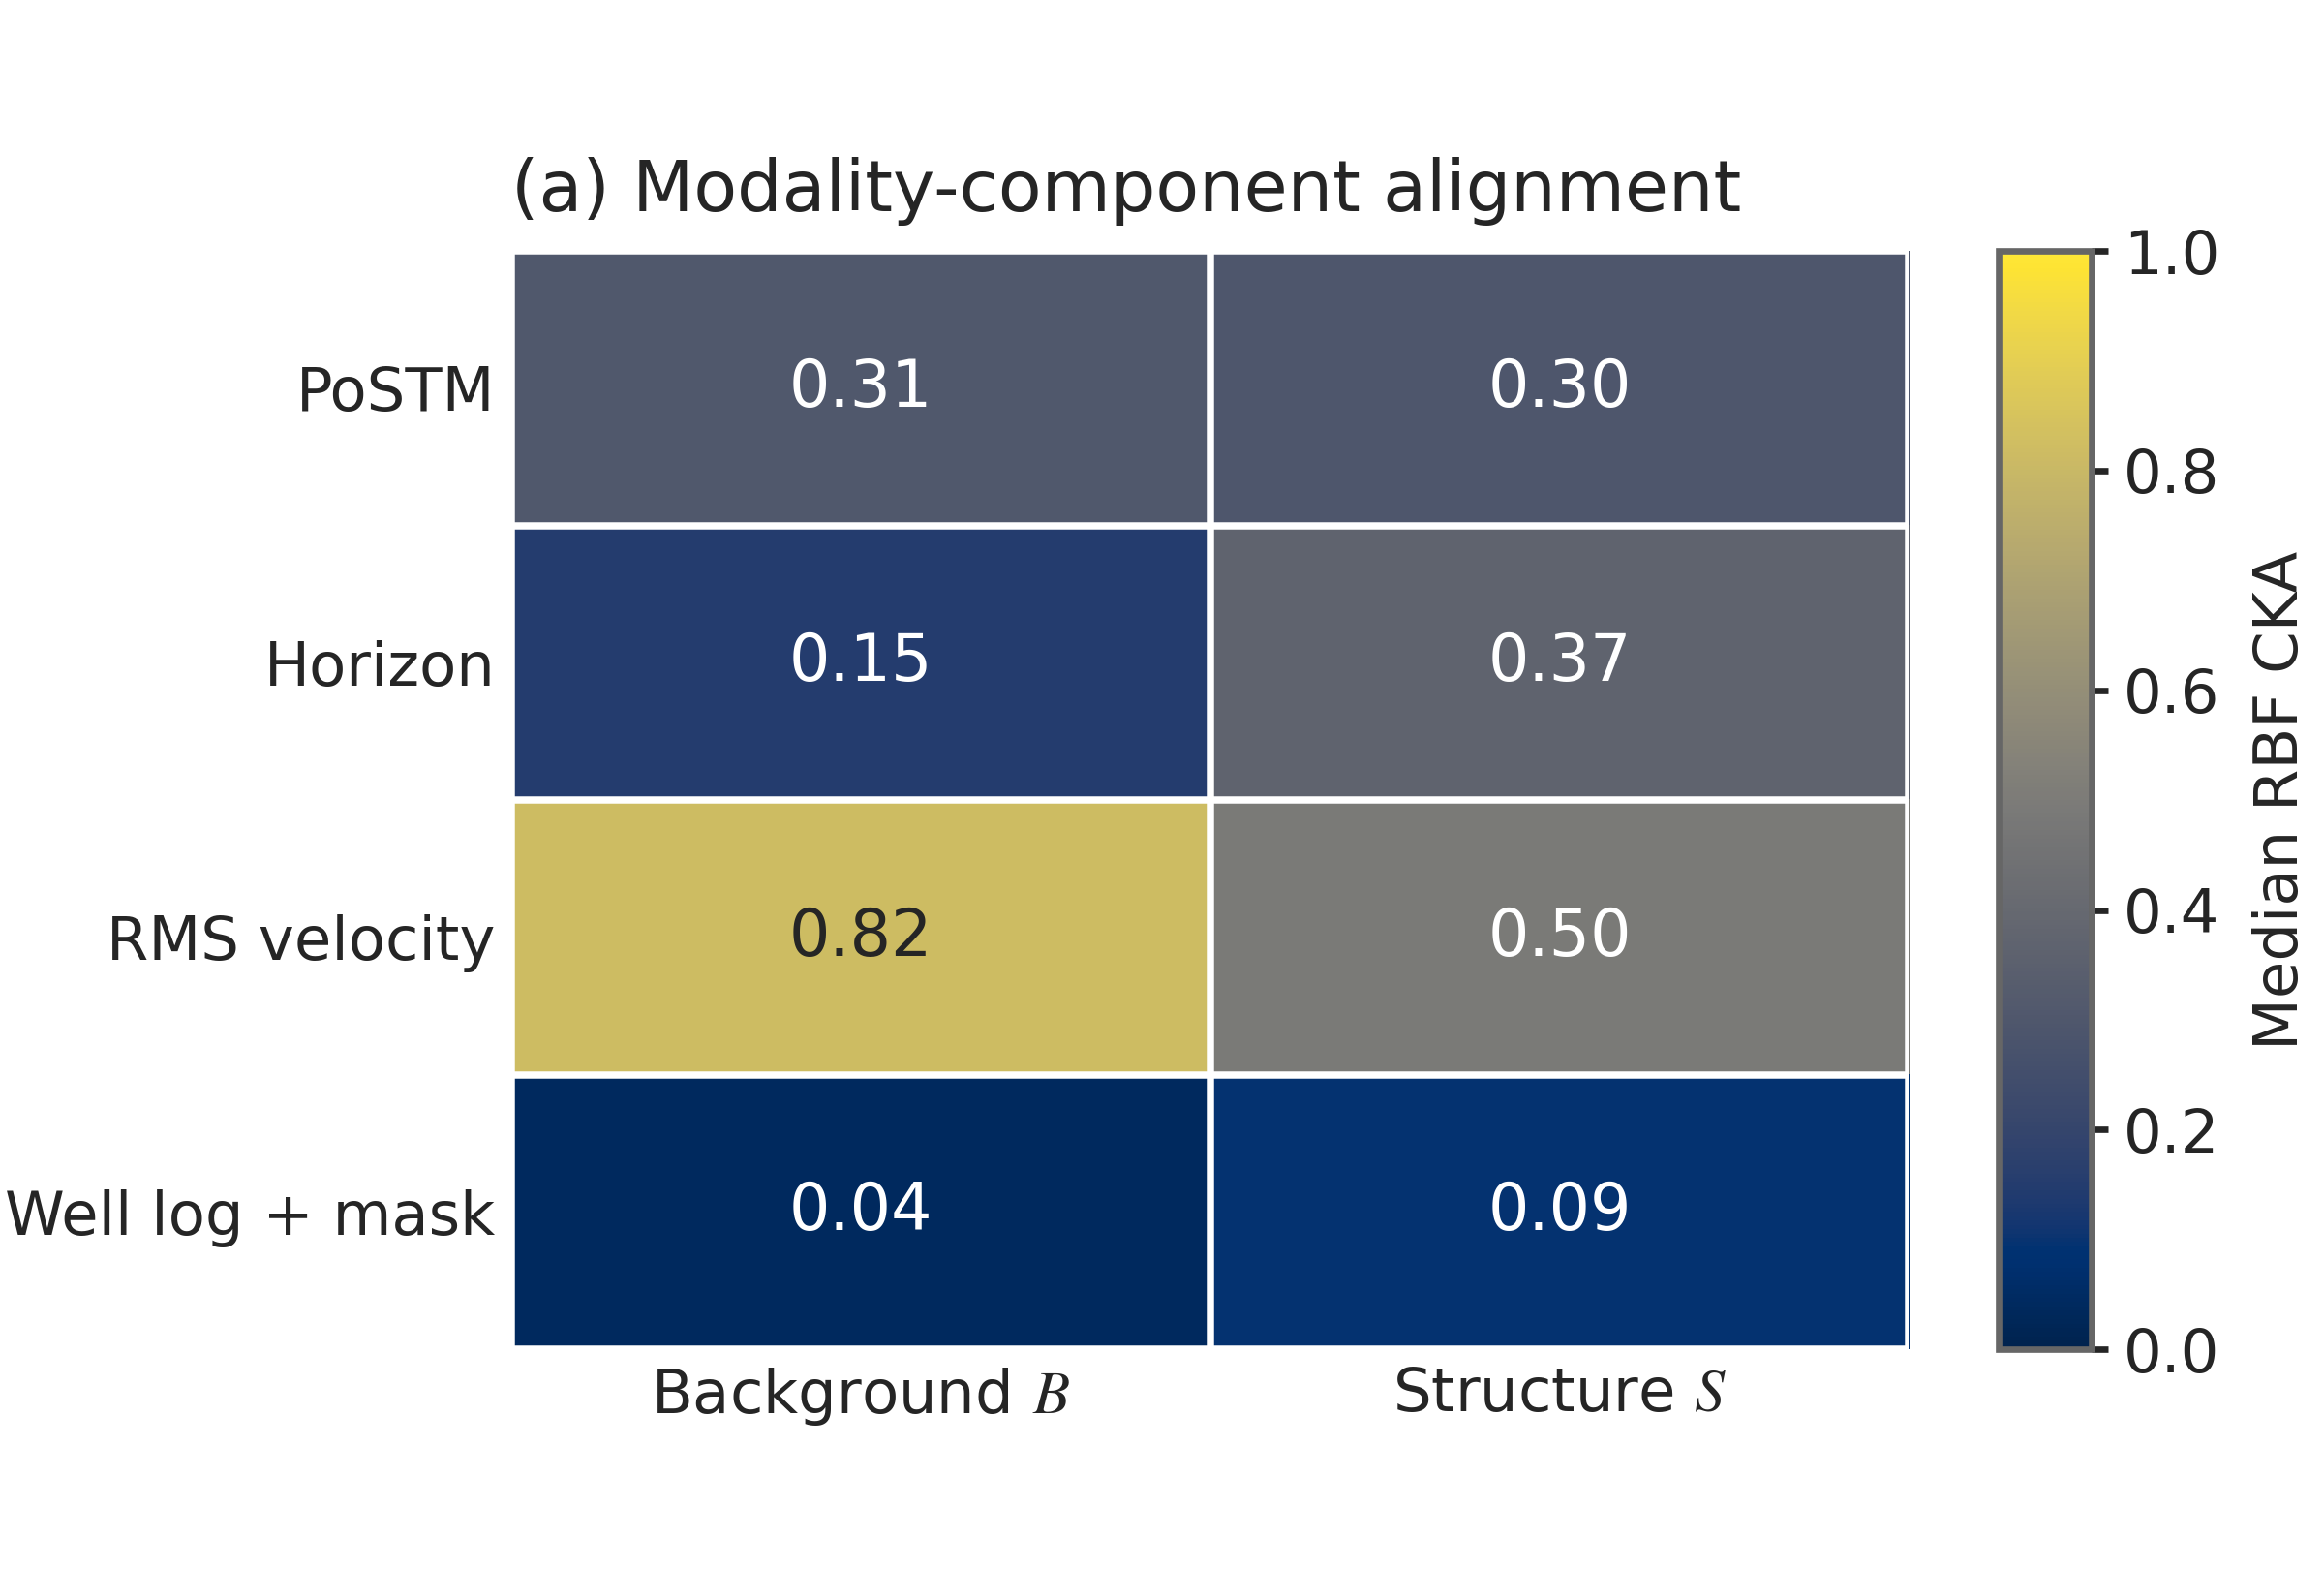
\includegraphics[width=\linewidth]{figures/modality_target_alignment_v2.png}\\[-2pt]
\textbf{(a)}
\end{minipage}
\hfill
\begin{minipage}[t]{0.48\fulllength}
\centering
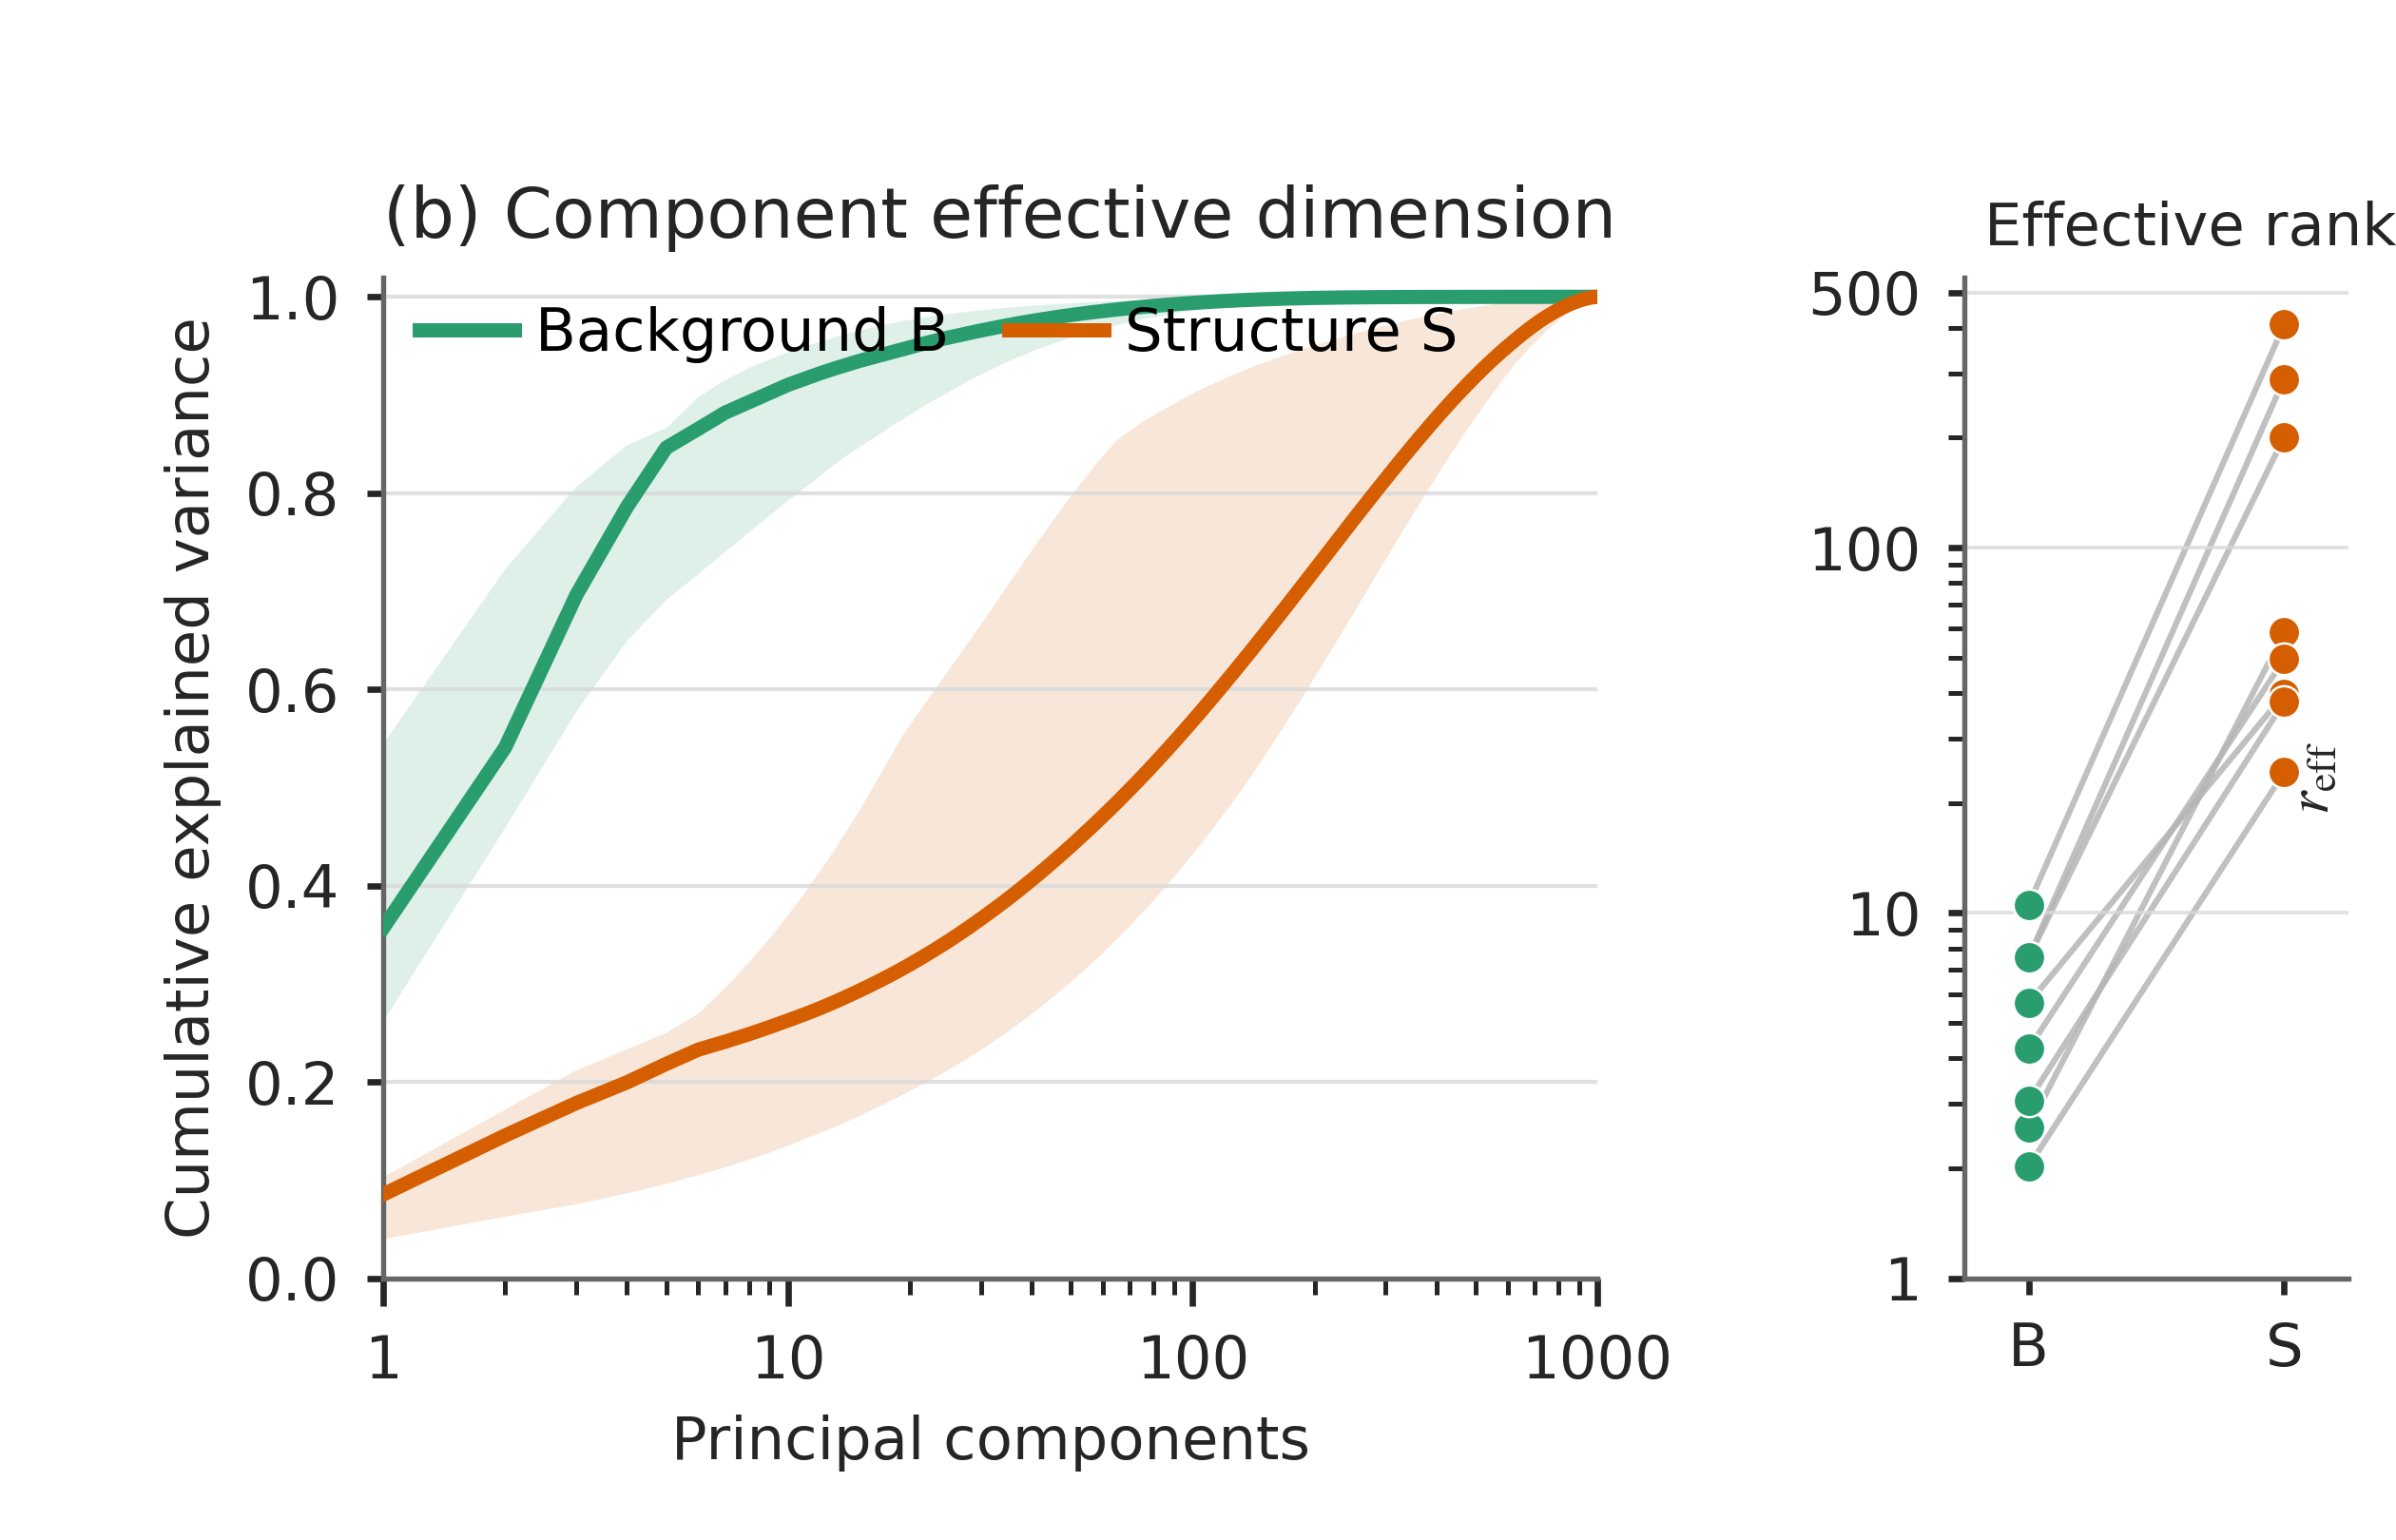
\includegraphics[width=\linewidth]{figures/component_effective_dimension_v2.png}\\[-2pt]
\textbf{(b)}
\end{minipage}
\caption{Training-set empirical characterization. (\textbf{a}) Modality-to-target alignment diagnostics summarize complementary tendencies of the four constraints. (\textbf{b}) Participation-ratio effective rank characterizes the smooth background and structural complement. These diagnostics motivate role-aware responsibility allocation but are not treated as proof of lower conditional complexity.}
\label{fig:data-characterization}
\end{figure}


\begin{figure}[H]
\centering
\begin{minipage}[t]{0.48\fulllength}
\centering
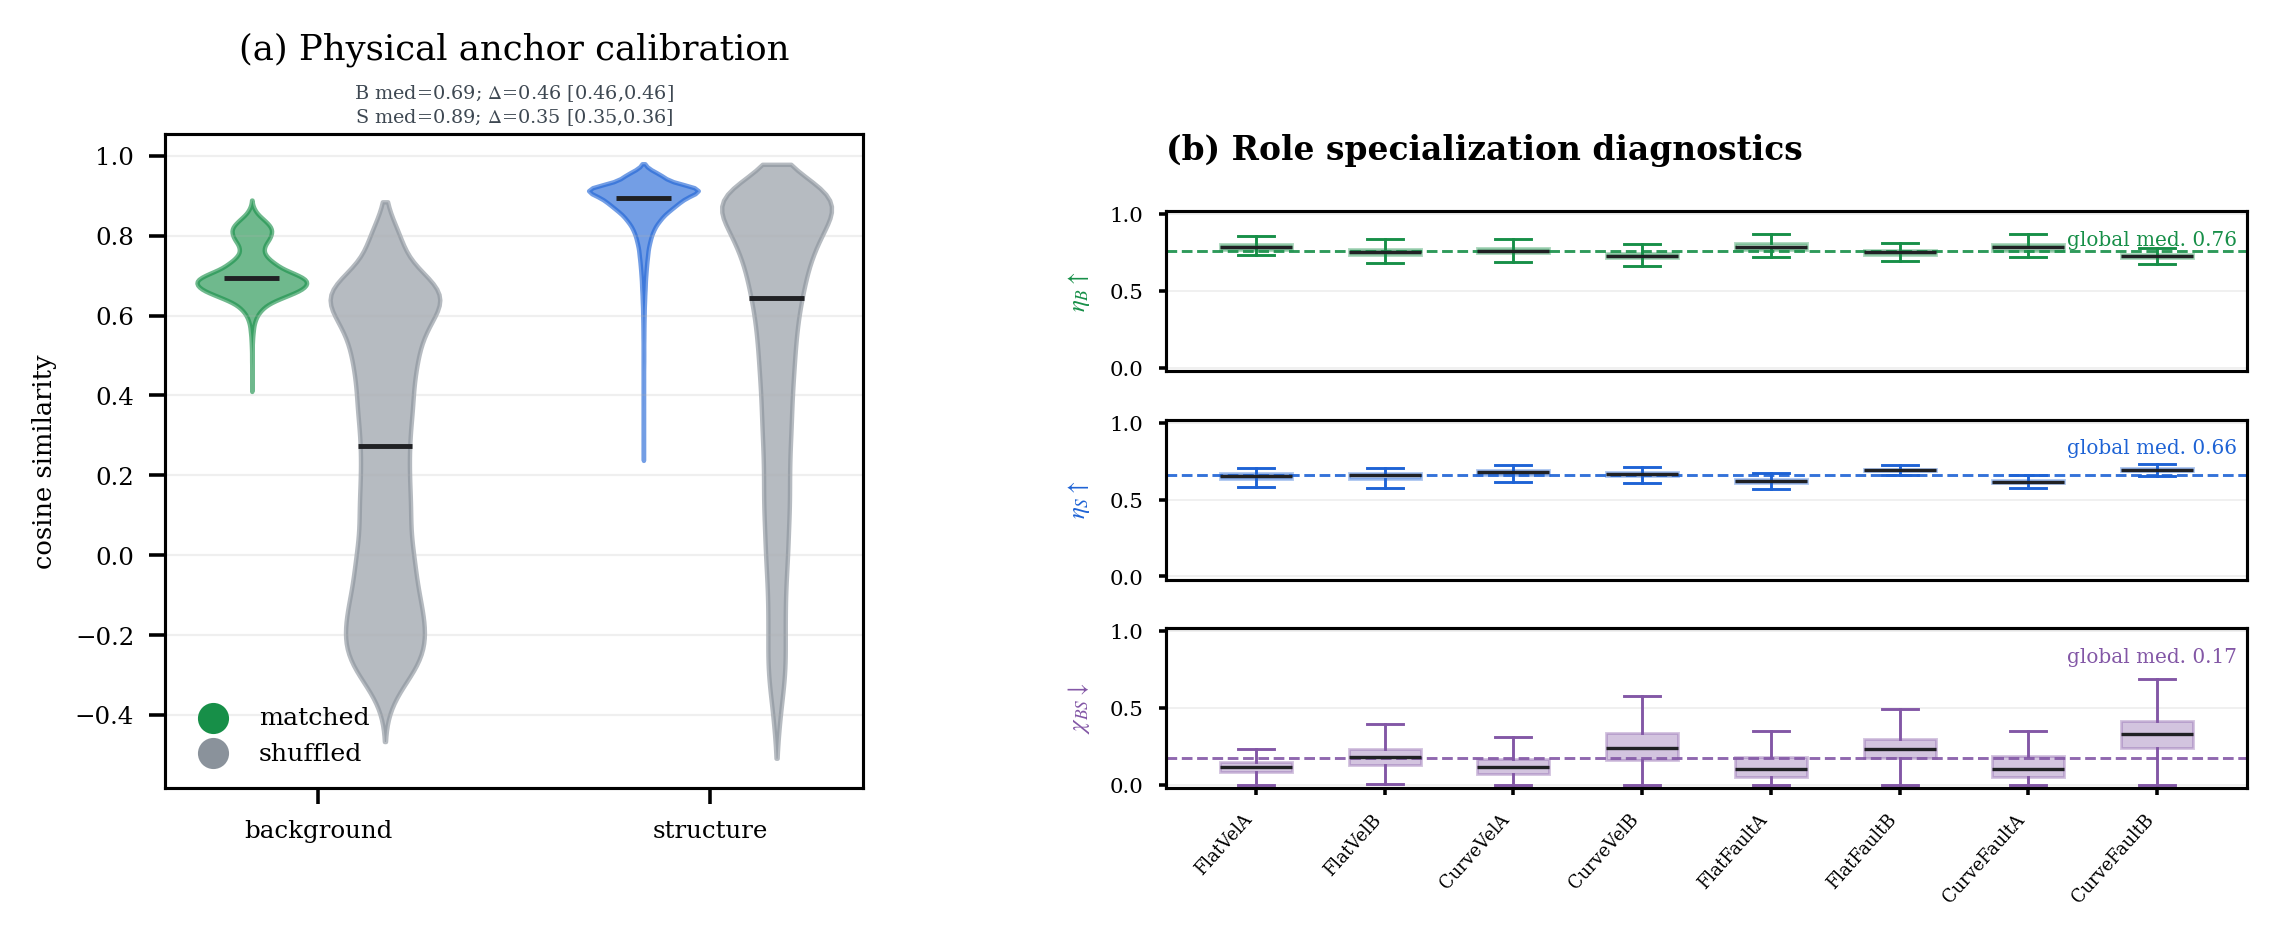
\includegraphics[width=\linewidth]{figures/figure3_condition_learning.png}\\[-2pt]
\textbf{(a)}
\end{minipage}
\hfill
\begin{minipage}[t]{0.48\fulllength}
\centering
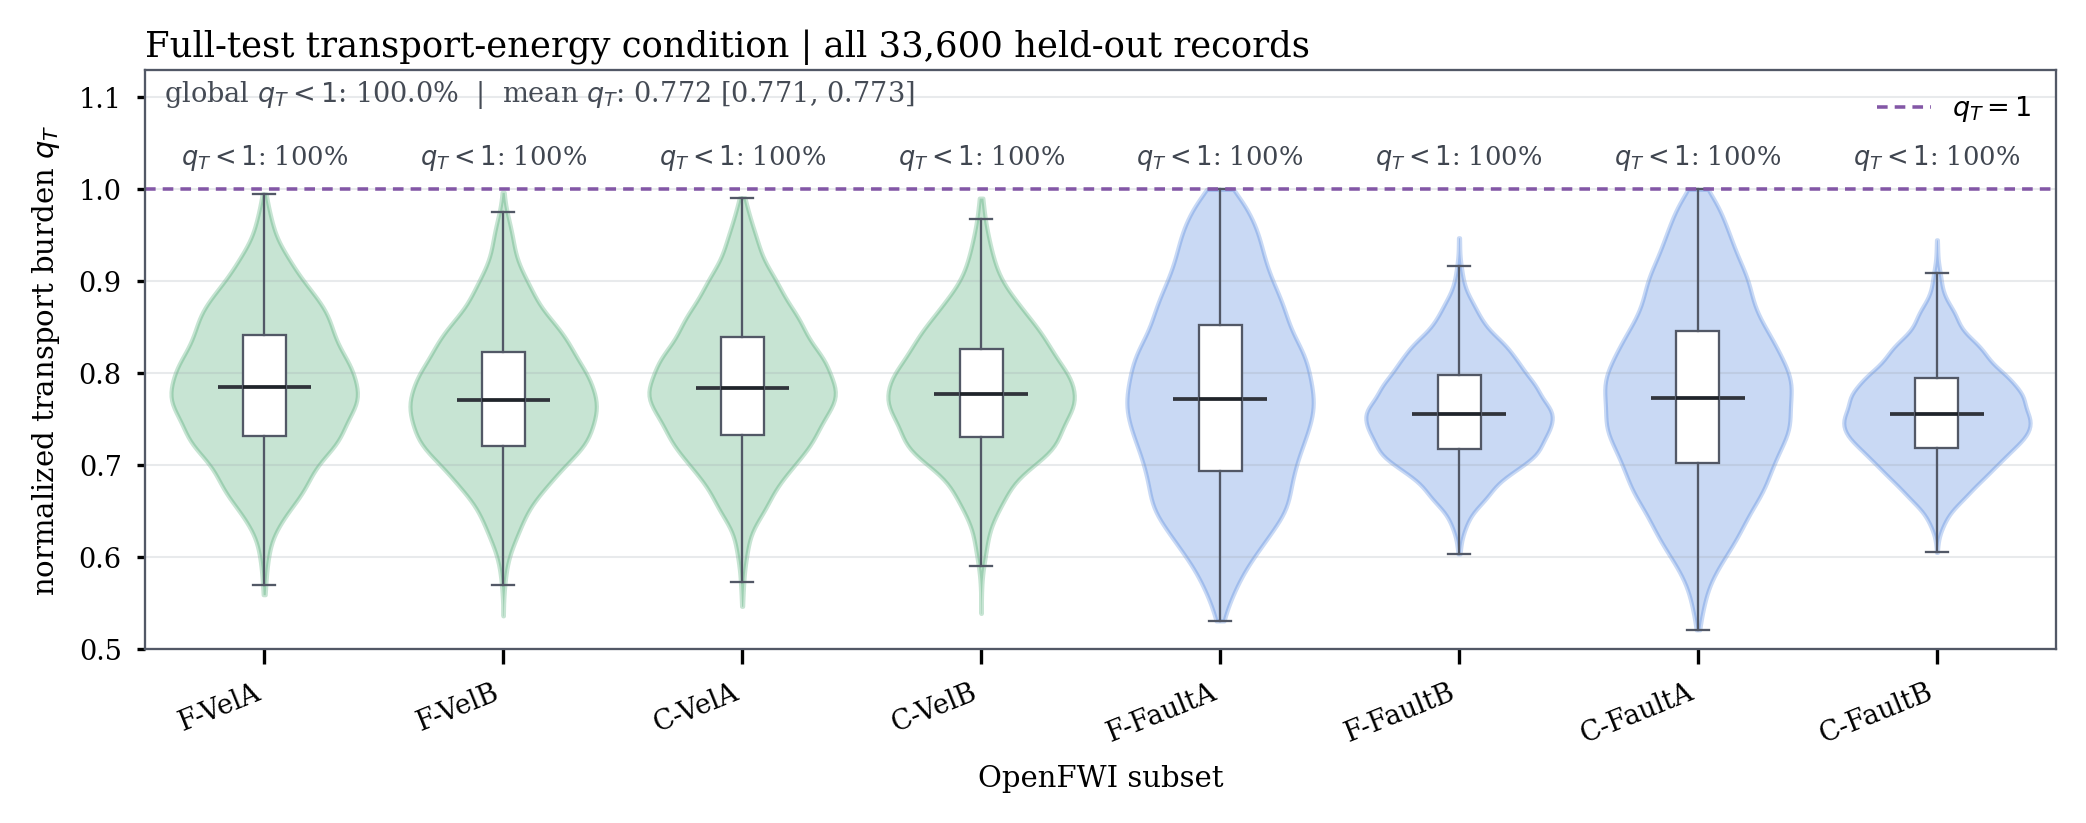
\includegraphics[width=\linewidth]{figures/figure4_residual_transport.png}\\[-2pt]
\textbf{(b)}
\end{minipage}
\caption{Diagnostics supporting interpretation of the model. (\textbf{a}) Condition-routing diagnostics characterize agreement of the learned role interfaces with their training-time anchors and intended frequency tendencies. (\textbf{b}) The normalized straight-path target-energy ratio $q_T$ characterizes the transport target after subtracting the predicted background. Both panels are empirical diagnostics rather than causal proofs of performance.}
\label{fig:diagnostics}
\end{figure}


Additional condition-routing details, the full effective-rank table, missing-modality stress tests, and extended qualitative panels are provided in the Supplementary Material.

\section{Discussion}

The central design choice in \method{} is to make reconstruction responsibility explicit. Multimodal inputs are not forced into a hard physical partition, but the learned condition interfaces feed two different downstream tasks. The background branch is optimized for direct estimation of a smooth velocity component, while the Flow Matching branch models the correction that remains relative to the predicted background. This differs from simply concatenating heterogeneous observations before a larger full-field predictor: the decomposition is operationally tied to which estimator is responsible for which part of the final model.

Prediction consistency is particularly important in this organization. If a residual model were trained relative to an oracle background $B$ but composed at inference with an imperfect estimate $\hat B$, the final reconstruction would contain a background mismatch that the residual model was never trained to correct. Defining the target as $V-\hat B$ and conditioning on the same $\hat B$ avoids that reference mismatch. Equation~\eqref{eq:rs_composition_identity} makes the error accounting explicit and provides a direct formulation-level justification without relying on stronger claims about entropy or intrinsic dimensionality.

The design analysis supports this interpretation. The controlled ablations show degradation when prediction consistency or background context is removed, while the complete configuration improves on fused and role-aware full-field Flow Matching within the historical ablation protocol. The diagnostic analyses provide complementary, but deliberately weaker, evidence. Effective-rank differences characterize the data decomposition; anchor-similarity margins characterize the learned role interfaces; and $q_T$ characterizes the residual transport target. None of these diagnostics is treated as a formal proof that the residual task is universally easier.

The unified comparison also clarifies the scope of the empirical claim. Latent U-Net achieves the strongest MAE, RMSE, and SSIM among the retained matched-input references, while InversionNet and the supervised multimodal UPFWI adaptation achieve lower MAE than BG-RFM. BG-RFM is therefore not presented as the overall accuracy winner. Its scientific contribution is the explicit reconstruction organization and prediction-consistent generative formulation, together with a compact parameterization that remains competitive under the common protocol.

The 10.6M-parameter footprint should be interpreted as an architectural property rather than a direct proxy for computational efficiency. BG-RFM uses fewer trainable parameters than the listed matched-input references, but the residual vector field requires repeated evaluations during ODE integration. Parameter count and wall-clock latency measure different properties, and faster inference is not claimed here.

The missing-modality experiments in Supplementary Section~S3 further show that the observation channels are not interchangeable. Removing sparse well information causes a moderate degradation, whereas removing horizon or RMS information has a much larger effect. In particular, the severe RMS-missing degradation is consistent with RMS velocity carrying essential large-scale velocity-scale information in this synthetic task. These stress tests support the complementary-observation interpretation but should not be extrapolated to field robustness.

The current study is intentionally bounded to synthetic, two-dimensional OpenFWI-derived models. Several constraints are constructed from the reference model to emulate processed or interpreted products, and their uncertainty is therefore more controlled than in field workflows. The study also does not establish three-dimensional deployment or downstream FWI/migration gains. Future work can replace idealized constraints with uncertain field interpretations, extend the formulation to 3D, and test whether the same responsibility allocation remains useful when observation quality and coverage vary more strongly.

\section{Conclusions}

We presented Background-Guided Residual Flow Matching (\method{}) for multi-constraint seismic velocity model building. The method learns role-aware conditions from RMS velocity, post-stack migrated images, interpreted horizons, and sparse wells, predicts a deterministic background velocity, and applies conditional Flow Matching to the correction relative to that prediction. The same predicted background connects residual supervision, residual conditioning, and final composition, creating a prediction-consistent reconstruction path.

Under the unified 33,600-record matched-input protocol, BG-RFM achieves an RMSE of 0.02695 and an SSIM of 0.99165 with 10.6M trainable parameters. The controlled design analysis further supports the roles of prediction consistency and background-conditioned residual transport, while the retained diagnostics characterize the background/structure decomposition and residual transport without being used as formal causal proof.

The resulting design expresses the central message of this study: predict the background and transport the prediction-relative correction. The evidence supports BG-RFM as a parameter-compact, structured formulation for integrating heterogeneous geophysical constraints in initial velocity model building, without requiring an overall benchmark-dominance claim.



%%%%%%%%%%%%%%%%%%%%%%%%%%%%%%%%%%%%%%%%%%
\ifdefined\BLINDREVIEW
\supplementary{A separate supplementary PDF accompanies the blind-review package.}
\authorcontributions{Administrative metadata withheld from the blind-review package.}
\funding{Administrative metadata withheld from the blind-review package.}
\institutionalreview{Not applicable.}
\informedconsent{Not applicable.}
\dataavailability{The study uses the publicly available OpenFWI benchmark. The multimodal observations are derived from OpenFWI using the processing and sampling procedures described in the manuscript.}
\acknowledgments{Administrative metadata withheld from the blind-review package.}
\conflictsofinterest{Administrative metadata withheld from the blind-review package.}
\else
\supplementary{A separate supplementary PDF contains the extended condition-learning objective, effective-rank characterization, missing-modality stress tests, additional diagnostics, baseline-adaptation details, and extended qualitative evidence.}
\authorcontributions{[ADMINISTRATIVE PLACEHOLDER --- provide the final CRediT author-contribution statement after author order is frozen.]}
\funding{[ADMINISTRATIVE PLACEHOLDER --- provide exact funder names, grant numbers, and APC funding statement, or confirm that the research received no external funding.]}
\institutionalreview{Not applicable.}
\informedconsent{Not applicable.}
\dataavailability{The study uses the publicly available OpenFWI benchmark \citep{deng2022openfwi}. The multimodal RMS-velocity, migrated-image, horizon, and sparse-well observations analyzed in this work are derived from the OpenFWI source data using the processing and sampling procedures described in the manuscript. Large processed arrays and checkpoints are not stored in the source repository. Source code, release configurations, data adapters, and evaluation utilities are available at \url{https://github.com/LT-xyh/seismic-diff-followup}. The exact submission revision will be archived or tagged before submission.}
\acknowledgments{[ADMINISTRATIVE PLACEHOLDER --- provide acknowledgments and, if required by the final confirmed use case, the MDPI-compliant generative-AI acknowledgment.]}
\conflictsofinterest{[ADMINISTRATIVE PLACEHOLDER --- confirm the final conflict-of-interest statement. If none: The authors declare no conflict of interest.]}
\fi

\reftitle{References}
\bibliography{references}
\end{document}
